\documentclass[12pt]{article}
\usepackage[utf8x]{inputenc}
\usepackage[a4paper, nohead, dvips, left=30mm, right=20mm, top=20mm, bottom=20mm]{geometry}
\usepackage[english, russian]{babel}
\usepackage[T1, T2A]{fontenc}
\usepackage{amsthm}
\usepackage{amssymb}
\usepackage{amsmath}
\usepackage{graphicx}
\usepackage{subfigure}
\usepackage{float}
\usepackage{array}
\usepackage[ruled]{algorithm}
\usepackage{algorithmic}
\usepackage{ulem}
\usepackage[usenames, dvipsnames]{color}

\graphicspath{{../figures/eps/bw/}}

\theoremstyle{plain}
\newtheorem{theorem}{Теорема}
\newtheorem{lemma}{Лемма}
\theoremstyle{definition}
\newtheorem{definition}{Определение}

\def\figureref#1{Рис.\,\protect\ref{#1}}
\def\eqref#1{(\protect\ref{#1}\protect)}

\def\RC{\hbox{root-code}}
\def\RCD{\hbox{root-code-decomp}}


\begin{document}
	\Russian

	\title{Перечисление $k$-танглов.}
	\author{В.\,Р.\,Мешков, А.\,С.\,Мишунин, А.\,В.\,Омельченко}

	\maketitle
	\tableofcontents

	\newpage
	\section{Введение}

		Целью настоящей работы является составление аналогичных уже известных для различных классов узлов и зацеплений таблиц неэквивалентных
		между собой $k$-танглов.

		\begin{definition}
			\label{definition:tangle}
			$k$-танглом называется гладкое вложение $k$ отрезков и конечного числа окружностей в $B^3$
			(трехмерный замкнутый шар единичного радиуса), если $2k$ концов отрезков взаимно однозначно отображаются
			на точки с координатами $(\cos\pi i/k, \sin\pi i/k, 0)$, $i\in\{0, 1, \dots, 2k{-}1\}$, называемые
			граничными точками $k$-тангла, и больше ни какие точки отрезков или окружностей на границу $B^3$ не отображаются.
		\end{definition}

		\begin{figure}[ht]
			\centering
			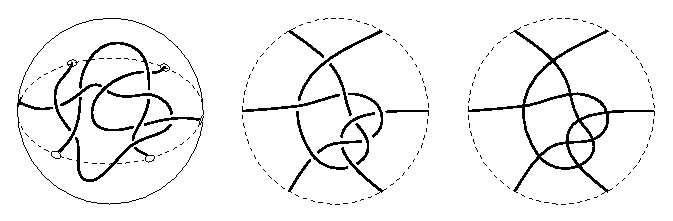
\includegraphics{c/tangle-diagram-projection.eps}
			\caption{\footnotesize $3$-тангл, его диаграмма и проекция\label{figure:3-tangle-and-proj}}
		\end{figure}

		Аналогично узлам и зацеплениям можно ввести понятие диаграммы и для $k$-танглов, строя невырожденные проекции $k$-тангла на плоскость,
		проходящую через концы его нитей, и снабжая их двойные точки информацией о расположении нитей, чьи проекции там пересеклись, по высоте.

		\begin{definition}
			\textit{Перекрестками} диаграммы (проекции) называются точки, в которые проецируются две точки $k$-тангла. \textit{Ребрами}
			диаграммы (проекции) называются максимальные множества точек, не лежащие на границе, в которые проецируется
			только по одной точке $k$-тангла. \textit{Граничными точками} диаграммы (проекции) называются проекции граничных точек $k$-тангла.
		\end{definition}

		Каждое из ребер диаграммы гомеоморфно открытому отрезку и соединяют либо 2 перекрестка, либо 2 граничные точки $k$-тангла
		либо граничную точку с перекрестком.

		Также нам понадабятся следующие определения:

		\begin{definition}
			Минимальной диаграммой $k$-тангла $T$ называют диаграмму $T$ с минимальным количеством перекрестков.
		\end{definition}

		\begin{definition}
			Диаграмма $k$-тангла называется альтернированной, если у каждого ребра, соединяющего два перекрестка, один из
			концов проходит над перекрестком, а другой --- под.
		\end{definition}

		\begin{definition}
			$k$-тангл называется альтернированным, если он имеет альтернированную диаграмму.
		\end{definition}

		\begin{figure}[ht]
			\centering
			\includegraphics{rational-and-4-tangle.eps}
			\caption{\footnotesize Рациональный тангл Конвея, $4$-тангл общего вида.\label{figure:rational-and-4-tangle}}
		\end{figure}

		Следует отметить, что танглы (точнее, $2$-танглы в смысле Определения~\ref{definition:tangle}) были введены
		в теорию узлов Дж.\,Конвеем в качестве средства для описания и классификации узлов~\cite{Conway1970}.
		Им же была предложено разделение $2$-танглов на
		классы рациональных, алгебраических и трансцендентных. Самым поддающимися исследованию оказались
		рациональные танглы~--- для них проблема классификации полностью
		решена~\cite{KauffmanLambropoulou2004}.

		Помимо результатов~\cite{KauffmanLambropoulou2004}, на настоящий момент в данной области имеются
		следующие достижения. Для простых альтернированных $2$-танглов получено полиномиальное уравнение на
		производящую функцию~\cite{SundbergThistlethwaite1998}. В~\cite{JustinZuber2003} и предшествующей
		серии статей для перечисления альтернированных $k$-танглов используются матричные интегралы;
		получены некоторые аналитические результаты, вычислены количества простых альтернированных $2$-{} и
		$3$-танглов с числом перекрестков до~11. Однако сложность предложенного метода быстро растет с
		увеличением $k$. Таким образом, практически все имеющиеся результаты касаются альтернированных
		$2$-танглов.

	\newpage
	\section{Перечисление проекций $k$-танглов}
	\label{section:projections}

	\subsection{Основные положения}
	\label{subsection:projection-statements}

		Первым шагом на пути к перечислению $k$-танглов может стать перечисление их проекций. Чтобы зря не усложнять себе задачу и
		уменьшить общее время работы алгоритма, примем следующие положения:
		\begin{enumerate}
			\item
			Мы не будем различать проекции (и диаграммы), различающиеся только плоской изотопией, сохраняющей гранцу диска,
			(деформацией)~--- весьма естественное условие.

			\item
			Мы также не будем различать проекции (диаграммы), отличающиеся гомеоморфизмом, сопровождающимся поворотом и/или отражением
			границы диска переводящим концы нитей друг в друга (иначе говоря, отличающиеся действием элемента диэдральной группы
			$D_{2k}$). Отличие таких проекций $k$-танглов друг от друга не слишком существенно и с топологической точки зрения
			естественно считать эквивалентными танглы, отличающиеся друг от друга лишь поворотом граничной окружности или зеркальным отражением;
			к тому же при больших $k$, учитывая, что большинство проекций несимметрично, в противном случае происходит увеличение их
			общего количества (а значит и времени работы алгоритма) практически в $4k$ раз. Следует заметить, что при перечислении
			аналитическими методами, подобными использованным в \cite{JustinZuber2003} и \cite{SundbergThistlethwaite1998}, не удается
			учесть наличие симметрий, вследствие чего некоторые танглы оказываются посчитанными в этом смысле несколько раз. Вычислительный
			подход позволяет устранить такие повторения.

			\item
			Мы будем рассматривать только простые проекции (диаграммы).
			\begin{definition}
				Диаграмма (проекция) $k$-тангла называется составной, если строго внутри граничной окружности существует замкнутая
				гладкая несамопересекающаяся кривая, которая трансверсально пересекает диаграмму ровно в двух точках и содержит
				внутри как минимум один перекресток. В противном случае проекция (диаграмма) называется простой. За примерами~---
				см.~\figureref{figure:composite-proj}.
			\end{definition}
			Исключение составных случаев несколько упрощает задачу без потери общности и обычно для теории узлов~\cite{Cromwell2004}.

			\item
			Мы будем рассматривать только связные проекции (диаграммы).
			\begin{definition}
				Диаграмма (проекция) называется \textit{связной}, если клеточный комплекс, составленный из перекрестков,
				граничных точек и ребер является линейно связным (см.~\figureref{figure:composite-proj}).
			\end{definition}
			Несвязные проекции содержательно не меняют дело, кроме того в противном случае число проекций и диаграмм для любого
			фиксированного количества перекрестков окажется бесконечным за счет возможности неограниченного добавления ни с чем
			не пересекающихся нитей.
		\end{enumerate}

		\begin{figure}[ht]
			\centering
			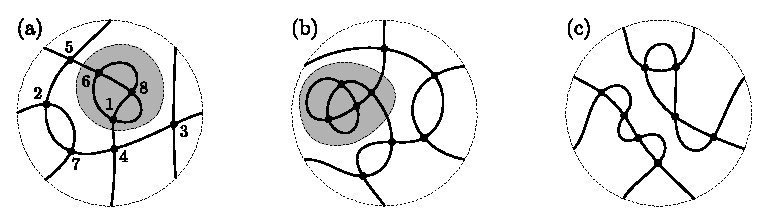
\includegraphics{c/composite-non-connected-projections.eps}
			\caption{\footnotesize Составные (a, b) и несвязная (c) проекции.\label{figure:composite-proj}}
		\end{figure}

		Алгоритм перечисления проекций вместе с доказательством корректности работы уже был подробно описан
		в~\cite{BogdanovMeshkovOmelchenkoPetrov2011}. В настоящем разделе мы напомним его важные для дальнейшего детали; затем мы покажем,
		как на его основе получить алгоритм для генерации альтернированных $k$-танглов, обладающий почти столь же хорошими свойствами, и,
		наконец, используем его вариацию для перечислния $k$-танглов с произвольными состояниями перекрестков.

		Подход, используемый для построения алгоритма перечисления проекций (и его обобщений), является частным случаем общей схемы,
		описанной в~\cite{McKay1998}
		под названием ``canonical construction path''. При этом подразумевается, что существует конечное и известное множество в некотором смысле
		``простейших'' объектов и множество преобразований-редукций во-первых, уменьшающих некоторый целочисленный полуинвариант рассматриваемых
		объектов, и во-вторых, позволяющих за конечное количество применений свести любой объект к одному из простейших. Основная идея метода~---
		сопоставить каждому из не ``простейших'' объектов каноническую редукцию, введя на объектах структуру бесконечного леса с корнями в
		``простейших'' объектах, и перечислять их в соответствии с полуинвариантом, обходя лес в глубину.

	\subsection{Элементарные операции с проекциями}
	\label{subsection:cutting}

		\begin{definition}
			Перекресток проекции назовем \textit{приграничным}, если он соединен одним из ребер проекции с
			одной из ее граничных точек.
		\end{definition}

		\begin{figure}[ht]
			\centering
			\subfigure{\includegraphics{tangle-border-deletion.1.eps}}
			\qquad
			\subfigure{\includegraphics{tangle-border-deletion.2.eps}}
			\qquad
			\subfigure{\includegraphics{tangle-border-deletion.3.eps}}
			\caption{\footnotesize Три варианта удаления пограничного перекрестка\label{figure:tangle-border-deletion}}
		\end{figure}

		\begin{definition}
			\textit{Удалением приграничного перекрестка} проекции называется операция, при которой выбранный
			перекресток удаляется из проекции вместе с ребрами, соединявшими его с граничными точками, а
			свободные концы ребер, ранее соединявших перекресток с другими перекрестками, становятся новыми
			граничными точками (\figureref{figure:tangle-border-deletion}). Число граничных точек может при этом меняться на
			$0$, $2$, или $-2$. Обратную операцию назовем \textit{приклеиванием приграничного перекрестка}. Любое удаление
			перекрестка, очевидно, уменьшает количество перекрестков диаграммы на единицу.
			Пограничный перекресток связной проекции, после удаления которого проекция теряет связность, мы будем в
			дальнейшем называть \textit{точкой сочленения}.
		\end{definition}

		Все точки сочленения можно найти с помощью модифицированного поиска в глубину, описанного в
		книгах~\cite{CormenLeisersonRivestStein2009, Sedgewick1983}.

		В статье~\cite{BogdanovMeshkovOmelchenkoPetrov2011} доказано, что любую простую связную проекцию можно, применяя
		операцию удаления, превратить в простейшую~--- проекцию с одним перекрестком (см.~\figureref{figure:geneology}), причем так,
		что все промежуточные проекции будут связными; иными словами, у любой связной проекции, имеющей более одного перекрестка, найдется
		пограничный перекресток, не являющийся точкой сочленения. Обратное также справедливо~--- любую простую связную проекцию можно получить
		из простейшей при помощи некоторой последовательности операций приклеивания. Подобное утверждение выполняется и для составных
		проекций, но простейшие здесь будут выглядеть уже по-другому.

		\begin{figure}[ht]
			\centering
			\includegraphics{sequential-border-deletion.eps}
			\caption{\footnotesize Сведение проекции к простейшей последовательными удалениями приграничных перекрестков\label{figure:geneology}}
		\end{figure}

		\begin{definition}
			Назовем некоторое свойство $X$ проекций $k$-танглов \textit{наследуемым}, если для любой проекции $T$ выполняется следующее:
			$\neg X(T) \Rightarrow \neg X(P)$ и $X(T) \Rightarrow X(N)$, где $P$~--- любая проекция, которую можно получить из $T$
			удалением пограничный перекрестков, и $N$~--- любая проекция, которую можно получить из $T$ приклеиванием пограничных
			перекрестков.
		\end{definition}

		Учитывая вышеизложенное, можно заметить, что, если $X$~--- наследуемое свойство, то любую проекцию, удовлетворяющую $\neg X$, можно
		получить из простейшей с помощью приклеиваний пограничных перекрестков так, что все промежуточные результаты удовлетворяют $\neg X$.
		Отметим, что свойство проекции быть составной является наследуемым.

		Исходя из сказанного, уже можно предложить следующий простой алгоритм перечисления. Пусть $P_n$~---
		множество всех связных простых проекций с $n$ перекрестками; так, например, множество $P_1$
		состоит из одного элемента~---  простейшей проекции:
		$P_1=\bigl\{\raise-0.4em\hbox{\includegraphics{simplest-projection.eps}}\bigr\}$. Имея $P_n$, построим
		множество $P_{n+1}$ следующим образом: возьмем мультимножество результатов всех возможных
		приклеиваний приграничного перекрестка ко всем проекциям из $P_n$ и удалим из него составные проекции. Затем удалим дубликаты.

		Последний шаг, к сожалению, является нетривиальным и, кроме того, существенно замедляет работу алгоритма. Далее мы избавимся
		от этого недостатка. Важным же здесь является способ, которым мы исключили составные проекции (а из наследуемости легко показать,
		что это действительно так). Заметим, что аналогичным образом мы можем избавится от всех проекций, удовлетворяющих какому-то
		наследуемому свойству. Этот факт нам понадобится при обобщениях.

	\subsection{Инвариант помеченных проекций}
	\label{subsection:root-code}

		\begin{definition}
			\textit{Помеченной проекцией} называется связная проекция $k$-тангла, снабженная тройкой
			$r=(v,e,f)$, где $v$~--- перекресток проекции, $e$~--- ребро проекции, инцидентное $v$, и $f$~---
			направление обхода (против часовой стрелки, или по часовой стрелке).
			Назовем $v$ \textit{помеченным перекрестком} и $e$~--- \textit{помеченным ребром}.
		\end{definition}

		Присвоим перекрестку $v$ номер 1, объявим первым входящим в него ребром ребро $e$, и сопоставим помеченной проекции список
		целых чисел согласно следующему алгоритму (см.~\figureref{figure:rcode-example}), являющемуся модификацией поиска
		в ширину (BFS)~\cite{CormenLeisersonRivestStein2009, Sedgewick1983}, одновременно вычисляя для всех остальных перекрестков
		номер и первое входящее ребро.

		\begin{algorithm}[ht]
			\footnotesize
			\caption{\small $\RC(P,(v,e,f)) $\label{algorithm:root-code}}
			\algsetup{linenosize=\small,linenodelimiter=.}
\begin{algorithmic}[1]
    \STATE $A \leftarrow \{\}$
    \STATE $free \leftarrow 2$
    \STATE $Q \leftarrow \{v\}$
    \STATE $number[v] \leftarrow 1$
    \STATE $incoming[v] \leftarrow e$
    \WHILE{$Q \neq \varnothing$}
        \STATE $u \leftarrow head[Q]$
        \STATE $dequeue(Q)$
        \FOR{(для) всех ребер $(u, w) \in P$ в порядке,\\ заданном $f$, начиная с $incoming[u]$}
            \IF{$w$ --- конец диаграммы}
                \STATE $code \leftarrow 0$
            \ELSE
                \IF{$number[w]$ не определен}
                    \STATE $number[w] \leftarrow free$
                    \STATE $free \leftarrow free + 1$
                    \STATE $enqueue(Q, w)$
                \ENDIF
                \STATE $code \leftarrow number[w]$
            \ENDIF
            \STATE $push(A, code)$
        \ENDFOR
    \ENDWHILE
    \RETURN $A$
\end{algorithmic}
		\end{algorithm}

		\begin{figure}[ht]
			\centering
			\subfigure{\includegraphics{root-code-example.1.eps}}
			\qquad
			\subfigure{\includegraphics{root-code-example.2.eps}}
			\caption{\footnotesize Примеры вычисления инварианта \RC\label{figure:rcode-example}}
		\end{figure}

		Результатом работы алгоритма является последовательность $A$, в которой на каждый перекресток
		проекции $P$ приходится 4~числа~--- номера соседних перекрестков в порядке обхода, заданном
		$f$ (для приграничных перекрестков на позициях, соответствующих граничным точкам, ставится $0$)
		начиная с вычисленного для этого перекрестка первого входящего ребра.
		Номера присваиваются перекресткам начиная с единицы в порядке появления в очереди обхода в ширину,
		первым входящим в перекресток (не $v$) ребром объявляется то, по которому мы впервые обнаружили данный
		перекресток. В последовательности $A$ перекрестки описаны также в порядке возрастания присвоенного номера.
		Для понятности примеры работы Алгоритма~\ref{algorithm:root-code} изображены на~\figureref{figure:rcode-example}.

		Легко понять, что по заданной последовательности указанного вида исходная проекция однозначно
		восстанавливается \cite{BogdanovMeshkovOmelchenkoPetrov2011}, следовательно одинаковым (гомеоморфным) помеченным
		проекциям соответствуют одинаковые последовательности, а разным~--- разные. Таким образом, последовательность $A$
		представляет собой \textit{инвариант} помеченных проекций; мы будем называть его \textit{root-code}.

		Определим теперь $\RC(P,v)$, соответствующий перекрестку $v$ проекции $P$ как лексикографически
		минимальный \RC{} среди всех восьми способов пометить проекцию $P$ с помеченной вершиной $v$.
		Заметим, что $\RC(P,v)=\RC(P,u)$ для $v\neq u$, $v,u\in P$ тогда и только тогда, когда проекция
		$P$ обладает нетривиальной группой симметрий, то есть существует автоморфизм (гомеоморфизм на
		себя, симметрия) проекции $P$, переводящий $v$ в $u$.

	\subsection{Алгоритм перечисления проекций}
	\label{subsection:projections-algorithm}

		\begin{figure}[ht]
			\centering
			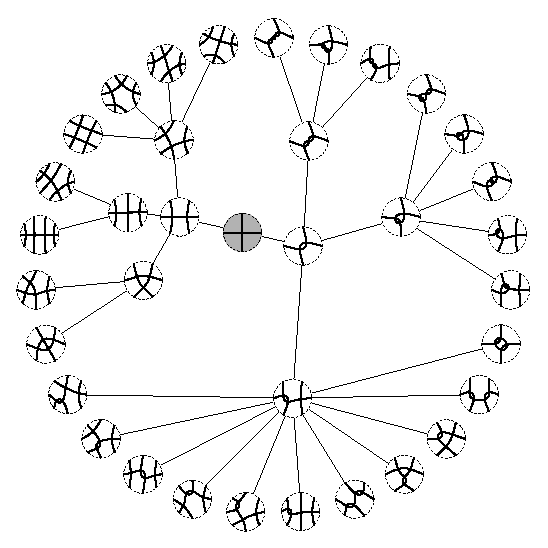
\includegraphics[width=77mm]{c/genealogical-tree.eps}
			\caption{\footnotesize <<Генеалогическое древо>> проекций\label{figure:genealogical-tree}}
		\end{figure}

		\begin{definition}
			Пусть $I=\raise-0.4em\hbox{\includegraphics{simplest-projection.eps}}$ --- простейшая проекция. Определим на
			множестве простых связных проекций $k$-танглов отображение $prev()$ со следующими свойствами:
			\begin{itemize}
				\item $prev(I)=\varnothing;$
				\item $prev(T)$, $T\ne I$, является результатом удаления из проекции $T$ приграничного
				перекрестка $v$, не являющегося точкой сочленения, такого что $\RC(T,v)$
				лексикографически минимален среди всех таких перекрестков.
			\end{itemize}
		\end{definition}

		Согласно результатам параграфа~\ref{subsection:cutting}, отображение $prev()$ определено на всем
		множестве простых связных проекций $k$-танглов. Оно однозначно благодаря тому, что все
		удовлетворяющие определению способы выбора перекрестка отличаются друг от друга автоморфизмом
		(см.~параграф~\ref{subsection:root-code}), следовательно все результаты удаления таких
		приграничных перекрестков гомеоморфны друг другу, а гомеоморфные проекции мы друг от друга не
		отличаем.

		Благодаря указанным свойствам, $prev()$ задает на множестве всех связных простых проекций
		структуру бесконечного дерева с корнем в $I$ (см.~\figureref{figure:genealogical-tree}). Для
		перечисления всех проекций с не более чем $n$ перекрестками достаточно обойти это дерево
		алгоритмом DFS (поиска в глубину) на глубину $n$
		(см.~Алгоритм~\ref{algorithm:projections-enumeration}). Единственный тонкий момент, который нужно
		учитывать, чтобы не спускаться по одному и тому же ребру несколько раз,~--- это возможное наличие
		нетривиальных симметрий у проекций.

		\begin{algorithm}[ht]
			\footnotesize
			\caption{\small DFS(T)\label{algorithm:projections-enumeration}}
			\algsetup{linenosize=\small,linenodelimiter=.}
\begin{algorithmic}[1]
    \PRINT $T$
    \IF{$crossings[T] = n$}
        \RETURN
    \ENDIF
    \STATE $list \leftarrow \varnothing$
    \FOR{(для) всех возможных результатов $R$\\приклеивания перекрестка $v$ к $T$}
        \IF{$R$ --- простая проекция}
            \IF{$prev(R) = T$}
                \STATE $r \leftarrow $ root-code($R$, $v$)
                \IF{ {\bf not} $contains(list, r)$}
                    \STATE DFS($R$)
                    \STATE $add(list, r)$
                \ENDIF
            \ENDIF
        \ENDIF
    \ENDFOR
\end{algorithmic}
		\end{algorithm}

		На самом деле, в этом алгоритме можно избавится от просеивания с помощью списка кодов (строчка 10) в каждой вершине дерева,
		а значит и от лишних вычислений, следующим образом: в процессе проверки в строчке 8 вместе с несколькими \RC{} вычислять группу
		симметрии проекции. Имея последнюю, можно сразу же сделать вывод, в каких позициях проверка из строчки 10 пройдет.

		К достоинствам такого подхода относятся полиномиальное от параметров задачи время в пересчете на одну проекцию, полиномиальный же
		общий расход памяти (отсутствие хеш-таблиц), практически идеальная возможность параллелизации (разные ветви дерева полностью
		независимы) и большой потенциал для обобщения.

		В качестве примера в Таблице~\ref{table:tangle-projections} приведены результаты работы Алгоритма~\ref{algorithm:projections-enumeration}.

		\begin{table}[ht]
			\caption{Количество проекций $k$-танглов с $n$ перекрестками.\label{table:tangle-projections}}
			\centering
			{\footnotesize
			\begin{tabular}{|c||r|r|r|r|r|r|r|r|r|r|r|r|}
			\hline
			$k$\textbackslash $n$
			    & 1 & 2 & 3 &  4 &   5 &   6 &      7 &       8 &        9 &          10 &           11 &            12 \\
			\hline\hline
			2   & 1 & 1 & 2 &  6 &  19 &  71 &    293 &  1\,348 &   6\,568 &     33\,701 &     178\,706 &      973\,085 \\
			3   & . & 1 & 2 &  8 &  29 & 138 &    638 &  3\,237 &  16\,805 &     90\,239 &     494\,151 &   2\,756\,453 \\
			4   & . & . & 2 &  8 &  41 & 210 & 1\,125 &  6\,138 &  34\,112 &    192\,278 &  1\,096\,560 &   6\,317\,363 \\
			5   & . & . & . &  5 &  31 & 231 & 1\,458 &  9\,183 &  56\,084 &    340\,885 &  2\,060\,224 &  12\,446\,400 \\
			6   & . & . & . &  . &  16 & 161 & 1\,406 & 10\,572 &  74\,331 &    499\,902 &  3\,276\,104 &  21\,112\,641 \\
			7   & . & . & . &  . &   . &  60 &    840 &  8\,818 &  75\,747 &    591\,091 &  4\,327\,816 &  30\,451\,898 \\
			8   & . & . & . &  . &   . &   . &    261 &  4\,702 &  56\,199 &    541\,570 &  4\,628\,641 &  36\,633\,417 \\
			9   & . & . & . &  . &   . &   . &      . &  1\,243 &  26\,753 &    361\,106 &  3\,846\,580 &  35\,758\,786 \\
			10  & . & . & . &  . &   . &   . &      . &       . &   6\,257 &    155\,593 &  2\,332\,512 &  27\,199\,662 \\
			11  & . & . & . &  . &   . &   . &      . &       . &        . &     32\,721 &     916\,595 &  15\,123\,600 \\
			12  & . & . & . &  . &   . &   . &      . &       . &        . &           . &     175\,760 &   5\,464\,661 \\
			13  & . & . & . &  . &   . &   . &      . &       . &        . &           . &            . &      963\,900 \\
			\hline
			all & 1 & 2 & 6 & 27 & 136 & 871 & 6\,021 & 45\,241 & 352\,856 & 2\,839\,086 & 23\,333\,649 & 195\,201\,866 \\
			\hline
			\end{tabular}
			}
		\end{table}

	\newpage
	\section{Перечисление альтернированных $k$-танглов}
	\label{section:alternating}

	\subsection{Альтернированные $k$-танглы}

		Напомним, что альтернированной называется такая диаграмма тангла (и, аналогично, узла или зацепления), в которой каждое
		ребро, имеющее перекрестки на обоих своих концах, с одной стороны проходи под перекрестком, а с другой~--- над перекрестком.
		Альтернированным называется $k$-тангл (узел, зацепление), имеющий альтернированную диаграмму.

		Как и в случае обычных альтернированных узлов и зацеплений, задача перечисления альтернированных $k$-танглов существенно
		проще общей задачи перечисления, что обусловлено следующими важными свойствами альтернированных диаграмм (обобщающими
		на танглы так называемые гипотезы Тейта для узлов и зацеплений~\cite{Tait1900}):
		\begin{enumerate}
			\item
			Любая простая альтернированная диаграмма $k$-тангла является минимальной, то есть у соответствующего тангла
			нет диаграммы с меньшим числом перекрестков.

			\item
			Все минимальные диаграммы простого альтернированного тангла могут быть получены друг из
			друга применением (возможно, многократным) преобразования, называемого ``flype''
			(см.~\figureref{figure:flype}).
		\end{enumerate}

		Первое из этих свойств гарантирует, что тангл, заданный альтернированной диаграммой с $n$ перекрестками, не может быть
		эквивалентен никакому танглу, заданному диаграммой с меньшим числом перекрестков, а второе свойство, известное для
		узлов и зацеплений как \textit{Tait flyping conjecture}, позволяет построить простой алгоритм проверки эквивалентности
		двух альтернированных танглов. Сами гипотезы Тейта были доказаны с помощью особых свойств полинома Джонса в
		работах~\cite{Kauffman1987, Murasugi1987_1, Murasugi1987_2, Thistlethwaite1987, Thistlethwaite1988,
		MenascoThistlethwaite1991, MenascoThistlethwaite1993}.

		\begin{figure}[ht]
			\centering
			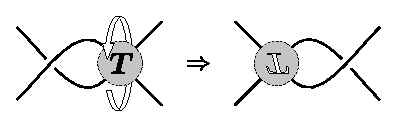
\includegraphics{c/flype.eps}
			\caption{\footnotesize Flype-преобразование, переворачивающее $2$-подтангл диаграммы\label{figure:flype}}
		\end{figure}

		Заметим, что в любой связной проекции существует только два способа расставить перекрестки альтернированным образом,
		и эти способы мы различать не будем, поскольку они порождают либо одинаковые, либо отличающиеся только зеркальным
		отражением $k$-танглы. Таким образом, альтернированные танглы мы можем рассматривать как подмножество множества проекций,
		содержащее по одному представителю из каждого класса эквивалентности по аналогичным flype-преобразованиям для проекций.
		Далее мы будем пытаться модифицировать вышеизложенный алгоритм для генерации данного подмножества проекций (здесь мы также
		примем положения из параграфа~\ref{subsection:projection-statements}). Нам понадобится несколько более сложный способ
		кодирования проекций, поэтому мы начнем с теоремы, следствиями которой будут важные свойства нового представления.

	\subsection{Теорема о пересекающихся танглах}

		Под словом ``тангл'' здесь мы будет подразумевать простую диаграмму $2$-тангла. Говоря ниже о танглах в терминах теории
		множеств, мы будем рассматривать их как множества перекрестков.

		\begin{theorem}
			\label{theorem:tangle-decomp-th}
			Пусть у нас есть два связных тангла $A$ и $B$, содержащиеся в какой-то простой диаграмме
			тангла или зацепления $D$. При этом $A\setminus B\neq\varnothing$, $B\setminus A\neq\varnothing$
			и $A\cap B\neq\varnothing$. Тогда $A\setminus B$, $B\setminus A$, $A\cap B$ и $A\cup B$ --- также связные
			танглы, а $A\cup B$ представим в виде (см. \figureref{figure:tangle-decomp}):

			\begin{figure}[H]
				\centering
				\includegraphics{tangle-decomp-theorem.eps}
				\caption{\footnotesize К Теореме \ref{theorem:tangle-decomp-th}\label{figure:tangle-decomp}}
			\end{figure}
		\end{theorem}
		\begin{proof}
			Обозначим за $a$ количество ребер, ведущих из $A\setminus B$ в остальную часть $D$. Аналогично за $b$ и $c$
			обозначим количество ребер, ведущих в остальную часть $D$ из $B\setminus A$ и из $A\cap B$ соответственно.
			Буквами $d$, $e$ и $f$ обозначим количество ребер между $A\setminus B$ и $A\cap B$, между $B\setminus A$ и
			$A\cap B$ и между $A\setminus B$ и $B\setminus A$ соответственно (см. \figureref{figure:tangle-decomp-proof}).
			Так как $A$ и $B$ --- танглы, то выполняются соотношения:
			\begin{equation}
				\label{equation:a_relation}
				a + c + e + f = 4
			\end{equation}
			\begin{equation}
				\label{equation:b_relation}
				b + c + d + f = 4
			\end{equation}
			Из того, что диаграмма $D$ --- простая, а также из того, что у любого $k$-тангла четное количество ног, следует:
			\begin{equation}
				\label{equation:ab_relation}
				d + e + c \ge 4
			\end{equation}
			\begin{equation}
				\label{equation:all_relation}
				a + b + c \ge 4
			\end{equation}
			\begin{equation}
				\label{equation:amb_relation}
				a + d + f \ge 4
			\end{equation}
			\begin{equation}
				\label{equation:bma_relation}
				b + e + f \ge 4
			\end{equation}
			\begin{figure}[H]
				\centering
				\includegraphics{tangle-decomp-proof.eps}
				\caption{\footnotesize К доказательству Теоремы \ref{theorem:tangle-decomp-th}\label{figure:tangle-decomp-proof}}
			\end{figure}

			Складывая попарно (\ref{equation:a_relation}) и (\ref{equation:b_relation}),
			(\ref{equation:ab_relation}) и (\ref{equation:all_relation}),
			(\ref{equation:amb_relation}) и (\ref{equation:bma_relation}), получаем соответственно:
			\[a + b + d + e + 2c + 2f = 8\]
			\[a + b + d + e + 2c \ge 8\]
			\[a + b + d + e + 2f \ge 8\]
			Отсюда следует, что $c = f = 0$, а все нестрогие неравенства на самом деле являются равенствами. В результате
			получаем систему линейных уравнений на $a$, $b$, $d$ и $e$, единственным решением которой является
			$a = b = d = e = 2$. Завершим доказательство, заметив, что для связности $A\setminus B$, $B\setminus A$ и
			$A\cap B$ достаточно простоты $D$.
		\end{proof}

	\subsection{Шаблоны, прямые суммы и макроперекрестки}
	\label{subsection:subtangle-decomposition}

		Для работы с классами flype-эквивалентности нам понадобится новое представление диаграмм $k$-танглов, подобное
		использованному для аналитического перечисления альтернированных $2$-танглов в~\cite{SundbergThistlethwaite1998}.
		Мы, однако, для тех случаев, где в~\cite{SundbergThistlethwaite1998} вводятся алгебраические шаблоны, будем использовать
		так называемые \textit{прямые суммы}~--- цепочки из двух или более $2$-танглов (см.~\figureref{figure:tangle-sum}).

		\begin{figure}[ht]
			\centering
			\includegraphics{tangle-sum.eps}
			\caption{\footnotesize Прямая сумма $T_1, T_2, \cdots, T_s$.\label{figure:tangle-sum}}
		\end{figure}

		Таким образом, каждую из диаграмм $k$-танглов мы будем представлять в виде некоторой специального вида проекции $k$-тангла
		с таким же количеством ног и с не большим, чем у исходной, количеством перекрестков, в каждом из которых содержится дополнительная
		информация о том, какой именно $2$-тангл и с какой ориентацией (поворотом, отражением, или и тем, и тем) нужно подставить вместо
		этого перекрестка, чтобы получить исходную диаграмму. Для этой специальной проекции у нас будет два возможный варианта: либо
		это просто цепочка из двух или более перекрестков (и тогда в результате подстановки из нее получится прямая сумма), либо это,
		как в работе~\cite{SundbergThistlethwaite1998}, \textit{базисный полиэдральный шаблон} (см.~\figureref{figure:template-tangles-decomposition}),
		или далее просто шаблон. Используемые здесь ``перекрестки'' с дополнительной информацией мы будем называть \textit{макроперекрестками}.
		Отметим, что диаграмму $k$-тангла с $k \ne 2$ невозможно представить в виде прямой суммы.

		\begin{figure}[ht]
			\centering
			\includegraphics{tangle-decomp-example.eps}
			\caption{\footnotesize Разложение на шаблон и $2$-танглы.\label{figure:template-tangles-decomposition}}
		\end{figure}

		Разумно теперь потребовать от нашего представления-разложения, чтобы оно, во-первых, было единственно, и, во-вторых, в случае
		шаблонов, чтобы оно было в некотором смысле максимально~--- то есть чтобы сам шаблон не допускал дальнейшего подобного разложения.
		И, если с прямыми суммами все понятно~--- достаточно потребовать, чтобы каждое из слагаемых не допускало разложение в прямую сумму
		в том же направлении (и тогда единственность немедленно следует из Теоремы~\ref{theorem:tangle-decomp-th}), то требования к
		разложению на шаблон с макроперекрестками мы формализуем следующим образом: в диаграмме $T$ каждому перекрестку $v$ сопоставим
		содержащийся в $T$ $2$-тангл $S(v)$ такой, что
		\begin{enumerate}
			\item
			$v \in S(v)$;

			\item
			$\forall R \subset T$, $R \ne T$, где $R$ --- $2$-тангл, $v \in R \Rightarrow R \subset S(v)$;

			\item
			$\forall u, u \in S(v) \Leftrightarrow S(u) = S(v)$.
		\end{enumerate}
		Отсюда получим искомое представление в виде шаблона и $2$-танглов по следующему правилу: каждому из непересекающхся множеств $S(v)$
		ставится в соответствие перекресток шаблона, в который вставлен непосредственно сам $2$-тангл $S(v)$, а ребрами шаблона становятся
		ребра исходной диаграммы, соединяющие разные множества $S(v)$. Единственность его немедленно следует из свойств 1--3; также заметим,
		что оно сохраняется под действием симметрий исходной диаграммы, и, более того, (чуть менее тривиальное, но весьма важное наблюдение)
		сохраняется под действием flype-преобразований в исходной диаграмме. Вопрос о существовании нам поможет разрешить
		Теорема~\ref{theorem:decomposition-existence}.

		\begin{theorem}
			\label{theorem:decomposition-existence}
			Любая простая связная диаграмма $k$-тангла представима либо в виде прямой суммы двух или более $2$-танглов, либо в виде
			шаблона с макроперекрестками, либо сама является одиночным перекрестком.
		\end{theorem}
		\begin{proof}
			Покажем, что любая удовлетворяющая условиям, не являющаяся одиночным перекрестком и не представимая в виде прямой суммы
			диаграмма представима в виде шаблона с макроперекрестками.
			
			Заметим, что всегда существует конфигурация,
			удовлетворяющая условиям 1 и 3~--- просто положим $S(v) = \{ v \}$. Пусть теперь у нас есть какие-то $S(v)$ для диаграммы
			$T$, удовлетворяющие условиям 1 и 3, но не удовлетворяющие условию 2, то есть в $T$ есть перекресток $v$ и $2$-подтангл
			$A \ne T$, для которых выполняется $v \in A$ и не выполняется $A \subset S(v)$. Тогда объединение $B$ всех $S(u)$ (а таких
			$S(u)$ больше одного), пересекающихся с $A$ будет $2$-танглом, что, полагая $S(u) = B$ для $\forall u \in B$, позволяет
			упростить наше разложение, уменьшив количество непересекающихся множеств. И вот по какой причине: конфигурация из $A$ и
			пересекающегося с ним, но не лежащего целиком внутри него $S(u)$ подходит под условия Теоремы~\ref{theorem:tangle-decomp-th},
			следовательно $A \cup S(u)$ представляет собой $2$-тангл; положим теперь $A = A \cup S(u)$ и продолжим рассматривать
			пересекающиеся с $A$ $S(u)$. Проделывая такое ``пополнение'' необходимое количество раз, мы покажем, что $B$~--- 2-тангл.

			Мы можем продолжать такое упрощение пока не выполнится условие 2, и тогда мы получим искомое разложение, либо пока не останется
			единственное множество $S(v)$. Но в последнем случае, поскольку мы упрощаем с помощью Теоремы~\ref{theorem:tangle-decomp-th},
			мы получим представление $T$ в виде прямой суммы.
		\end{proof}

		Напоследок отметим, что разложение в прямую сумму из точно двух минимальных слагаемых, вообще говоря, удовлетворяет условиям 1--3, но
		такие случаи мы к шаблонам относить не будем.

	\subsection{Инвариант нового представления}
	\label{subsection:root-code-decomp}

		Обобщим теперь наш инвариант \RC{} из параграфа~\ref{subsection:root-code} на новое представление. Как уже было сказано выше,
		шаблон (и структура прямой суммы, очевидно, тоже) сохраняется при симметриях диаграммы. Таким образом, новый инвариант должен
		так же, как и старый, учитывать внешнюю структуру (шаблона, или прямой суммы) и, кроме того, в каждом перекрестке должна учитываться
		информация о содерхащемся там $2$-тангле и его ориентации относительно входящего в перекресток ребра и глобального направления обхода.

		Алгоритм~\ref{algorithm:root-code-decomp}, на котором для удобства выделены изменения, строит новый инвариант. Введены новые
		обозначения: функция $tangle$, сопоставляющую каждому перекрестку $u$ число $tangle(u)$~--- неотрицательный номер содержащегося там
		$2$-тангла, и функцию $orientation(u,e,f)$~--- целое число от 0 до 7, кодирующее ориентацию $2$-тангла, содержащегося в $u$ относительно
		входящего в $u$ ребра $e$ и направления обхода $f$. На перекрестке $u$ с группой симметрии $G(u)$ $orientation$ может принимать
		$|\frac{D_4}{G(u)}|$ различных значений.
		
		\begin{algorithm}[ht]
			\footnotesize
			\caption{\small root-code-decomp$(P, (v, e, f))$\label{algorithm:root-code-decomp}}
			\algsetup{linenosize=\small, linenodelimiter=.}

			{\color{Gray}
			\begin{algorithmic}[1]
\STATE $A \leftarrow \{\}$
\STATE $free \leftarrow 2$
\STATE $Q \leftarrow \{v\}$
\STATE $number[v] \leftarrow 1$
\STATE $incoming[v] \leftarrow e$
\WHILE{$Q \neq \varnothing$}
    \STATE $u \leftarrow head[Q]$
    \STATE $dequeue(Q)$

    \STATE \textcolor{Black}{$push(A, tangle(u))$}

    \FOR{(для) всех ребер $(u, w) \in P$ в порядке,\\заданном $f$, начиная с $incoming[u]$}
        \IF{$w$ --- конец диаграммы}
            \STATE $code \leftarrow 0$
        \ELSE
            \IF{$number[w]$ не определен}
                \STATE $number[w] \leftarrow free$
                \STATE $free \leftarrow free + 1$
                \STATE $enqueue(Q, w)$
            \ENDIF
            \STATE $code \leftarrow number[w]$
        \ENDIF

        \STATE $push(A, code)$
    \ENDFOR

    \STATE \textcolor{Black}{$push(A, orientation(u, incoming[u], f))$}
\ENDWHILE
\RETURN $A$
			\end{algorithmic}
			}
		\end{algorithm}

		Мы специально потребуем, чтобы у тангла из одного перекрестка был минимально возможный номер 0, что гарантирует, что новый
		инвариант, вычисленный из перекрестка с подставленным простейшим $2$-подтанглом, будет гарантированно лексикографически меньше,
		чем вычисленный из любого другого перекрестка ~--- это свойство окажется удобным в дальнейшем.

		Отметим также, что для всех альтернированных диаграмм $k$-танглов, не раскладывающихся в прямую сумму, наш новый инвариант
		будет учитывать flype-эквивалентность, то есть будет полным.

	\subsection{Обобщение алгоритма перечисления}

		Свойство проекции $k$-тангла быть шаблоном, то есть не допускать нетривиального разложения как в
		параграфе~\ref{subsection:subtangle-decomposition}, в некотором смысле аналогично свойству простоты. Более того, свойство
		проекции не быть шаблоном~--- наследуемое, как и свойство быть составной. Таким образом, алгоритм перечисления проекций из
		параграфа~\ref{subsection:projections-algorithm} очень легко видоизменяется для перечисления шаблонов: единственное, что нужно
		добавить --- проверку на то, не появилось ли у проекции нетривиальное разложение на $2$-танглы и не образовали ли мы прямую сумму,
		при каждом приклеивании перекрестка.

		\begin{figure}[ht]
			\centering
			\includegraphics{tangle-to-graph.eps}
			\caption{\footnotesize Сопоставления планарного графа проекции $k$-тангла.\label{figure:tangle-to-graph}}
		\end{figure}

		После приклеивания перекрестка образовавшийся нетривиальный $2$-тангл может либо не содержать новый перекресток, либо содержать.
		От первого случая мы избавляемся очевидным запретом приклеивать что-либо к проекции, содержащей более одного перекрестка и
		имеющей четыре граничные точки. Второй случай проверяется следующим образом: сопоставим проекции граф как показано
		на~\figureref{figure:tangle-to-graph}. Каждому ребру полученного графа присвоим единичную пропускную способность, кроме случая,
		когда у проекции четыре граничные точки~--- тогда самому далекому от только что приклеенной вершины граничному ребру дадим
		бесконечную пропускную способность. Назначим истоком вершину, соответствующую границе проекции и стоком~--- вершину, соответствующую
		последнему приклеенному перекрестку. Легко показать, что максимальный поток в такой сети будет равен четырем, и проекция не содержит
		нетривиального $2$-подтангла тогда и только тогда, когда все вершины, кроме стока, достижимы из истока по остаточной сети
		максимального потока~\cite{CormenLeisersonRivestStein2009, Sedgewick1983}.

		Предположим, что у нас есть полный набор альтернированных $2$-танглов с числом перекрестков до $n$ и с информацией об их группах
		симметрии с учетом flype-эквивалентности. Сделаем еще одно несложное обобщение алгоритма: если раньше мы начинали с единственной
		проекции из одного перекрестка и действовали тремя возможными приклеиваниями перекрестков, то теперь на каждый $2$-тангл у нас
		будет по макроперекрестку, в каждом из которых $2$-тангл $T$ можно ориентировать $|\frac{D_4}{G(T)}|$ способами и приклеить,
		как и раньше, тремя способами, а начинать мы будем с множества проекций, состоящих из одного макроперекрестка каждого типа.

		Таким образом, у нас есть алгоритм перечисления альтернированных $k$-танглов. Единственной проблемой осталось получение $2$-танглов
		с точностью до flype-эквивалентности, а точнее $2$-танглов, разлагающихся в прямую сумму, поскольку остальные $2$-танглы мы
		получаем в процессе работы нашего алгоритма, и с некоторыми техническими ухищрениями, касающимися порядка обхода и хранения в памяти
		некоторого множества диаграмм, можем их там же и использовать.

	\subsection{Перечисление прямых сумм}

		Теперь нам остается откуда-то взять $2$-танглы, допускающие разложение в прямую сумму. Эту проблему мы будем решать, добавляя
		дополнительные ветви в древовидную структуру на шаблонах, используемую в алгоритме из предыдущего параграфа. Здесь, однако,
		нам надо будет разобраться со следующими тонкими моментами: во-первых, собираемые цепочки из макроперекрестков действительно
		должны быть прямыми суммами слагаемых, не допускающих дальнейшего разложения в прямую сумму в том же направлении. Для этого в
		каждом макроперекрестке мы должны хранить дополнительную информацию о разложимости исходного для него $2$-тангла в прямую
		сумму и учитывать эту информацию во время сборки. Во-вторых, если среди слагаемых в прямой сумме есть одиночные перекрестки,
		мы должны учитывать flype-эквивалентность, влияющую не только на количество различных $2$-танглов, но и на группу симметрии
		каждого из них. Таким образом прямые суммы играют для альтернированных $k$-танглов ту же роль, что flype-орбиты
		из~\cite{RankinSchermannSmith2002_1, RankinSchermannSmith2002_2, RankinSmith2002} для альтернированных узлов и зацеплений.

		\begin{figure}[ht]
			\centering
			\includegraphics{one-side-crossings.eps}
			\caption{\footnotesize Свободные перекрестки с одной стороны.\label{figure:one-side-crossings}}
		\end{figure}

		Заметим, что с помощью flype-преобразований в прямой сумме всегда можно собрать одиночные (или свободные) перекрестки по одну
		сторону от всех остальных слагаемых как на~\figureref{figure:one-side-crossings}. Также заметим важный факт: свойство конфигурации
		нарушать такое положение свободных перекрестков является наследуемым (относительно операций приклеивания дополнительных
		слагаемых, которыми мы здесь и пользуемся, разумеется). Таким образом мы можем избавится от значительной части дубликатов,
		связанных с flype-эквивалентностью, просто отсекая некоторые ветви, соответствующие другим положениям свободных перекрестков,
		в нашем дереве по простым правилам, приведенным в Таблице~\ref{table:sums-rules}. Здесь действие зависит от типов
		приклеиваемого перекрестка и самого близкого и самого далекого от приклеиваемого перекрестков суммы (в некоторых случаях два
		последних являются одним и тем же перекрестком).

		\begin{table}[ht]
			\caption{Правила сборки прямых сумм.\label{table:sums-rules}}
			\centering
			\begin{tabular}{cm{26mm}l}
				\hline\hline
				1 & \includegraphics{alternating-build-4-case.1.eps} & --- принять \\
				\hline
				2 & \includegraphics{alternating-build-4-case.2.eps} & --- принять \\
				\hline
				3 & \includegraphics{alternating-build-4-case.3.eps} & --- сравнить \\
				\hline
				4 & \includegraphics{alternating-build-4-case.4.eps} & --- отвергнуть \\
				\hline
				5 & \includegraphics{alternating-build-4-case.5.eps} & --- отвергнуть \\
				\hline
				6 & \includegraphics{alternating-build-4-case.6.eps} & --- отсекается инвариантом \\
				\hline
				7 & \includegraphics{alternating-build-4-case.7.eps} & --- принять \\
				\hline
				8 & \includegraphics{alternating-build-4-case.8.eps} & --- отсекается инвариантом \\
				\hline\hline
			\end{tabular}
		\end{table}

		Единственным оставшимся произволом в ситуации как на~\figureref{figure:one-side-crossings}, остается то, с какой из двух
		сторон окажется блок из одиночных перекрестков от блока из всех остальных слагаемых (а все остальные слагаемые ведут себя
		именно блоком, так как, в зависимости от четности числа свободных перекрестков, при ``глобальном'' flype-преобразовании
		либо не меняется, либо переворачивается как целое, а все симметричные друг другу конфигурации мы не различаем). Для
		разрешения этой ситуации нам оказывается полезным уже упоминавшееся в параграфе~\ref{subsection:root-code-decomp}
		свойство минимальности кода одиночного перекрестка, благодаря которому случаи 6 и 8 из Таблицы~\ref{table:sums-rules}
		никогда не встречаются. Таким образом, сторона, с которой будут свободные перекрестки, полностью определяется при
		рассмотрении случая 3. Для полного решения проблемы flype-эквивалентности нам остается выбрать в случае 3 из двух возможных
		приклеиваний одиночного перекрестка дающее минимальный \RCD{}.

		\begin{figure}[ht]
			\centering
			\includegraphics{d4-group-basis.1.eps}
			\qquad
			\includegraphics{d4-group-basis.2.eps}
			\caption{\footnotesize Базис группы $D_4$.\label{figure:d4-group-basis}}
		\end{figure}

		Для работы алгоритма нам также необходимо знать группы симметрии $2$-танглов, каждая из которых является одной из 10
		подгрупп диэдральной группы $D_4$. Далее для обозначения элементов $D_4$ мы выберем базис из поворота против часовой
		стрелки $C$ и отражения относительно пары противоположных граничных точек $E$ (см.~\figureref{figure:d4-group-basis}).

		В случае $2$-танглов, собранных по шаблону, задача определения группы симметрии решается следующим образом: с помощью
		вычисления инварианта проверяется симметричность относительно нескольких элементов $D_4$, а затем
		согласно~\figureref{figure:D4-subgroups} устанавливается подходящая подгруппа. В случае же с прямыми суммами, возможными
		симметриями являются поворот на $\frac{\pi}{2}$ и два отражения, меняющие местами пары граничных точек, на которые нам
		нужно проверить и саму диаграмму, и ее вариант с противоположным положением одиночных перекрестков (разумеется, если
		таковые присутствуют).

		\begin{figure}[ht]
			\centering
			\includegraphics{d4-subgroups.eps}
			\caption{\footnotesize Решетка подгрупп группы $D_4$.\label{figure:D4-subgroups}}
		\end{figure}

		Таким образом общая схема алгоритма перечисления альтернированных $k$-танглов с не более чем $n$ перекрестками выглядит
		следующим образом: на первом этапе мы работаем только с теми диаграммами, из которых могут получится $2$-танглы (такие
		диаграммы находятся в ``треугольнике'' по числу ног и числу перекрестков, в качестве примера в
		Таблице~\ref{table:alternating-tangles-table} соответствующие числа подчеркнуты). В процессе работы мы сохраняем все
		полученные диаграммы в память, и, когда обнаруживаем новый $2$-тангл, добавляем его в множество макроперекрестков со всей
		необходимой дополнительной информацией, пробегаясь по множеству сохраненных диаграмм и пробуя приклеить новый макроперекресток к
		каждой из них. Получив таким образом множество альтернированных $2$-танглов, мы переходим ко второму этапу~--- полностью
		аналогично алгоритму для проекций генерируем все оставшиеся альтернированные $k$-танглы.

		По сравнению с алгоритмом для проекций мы получили первую стадию, которая требует существенного количества памяти и не допускает
		простого распараллеливания, однако количество диаграмм, обрабатываемых на первой стадии, очень мало по сравнению с их полным
		количеством, как можно видеть в Таблице~\ref{table:alternating-tangles-table}.

	\subsection{Результаты}

		В качестве примера работы описанного алгоритма мы сгенерировали $k$-танглы с числом перекрестков до 12 включительно.
		Для проверки были также посчитаны количества альтернированных $2$-танглов без учета поворотов и отражений (для этого
		каждую диаграмму $T$ нужно учесть $\frac{8}{G(T)}$ раз). Результаты этих вычислений представлены в
		Таблице~\ref{table:old-results-table}, и они полностью согласуются с производящей функцией~\cite{SundbergThistlethwaite1998}.

		\begin{table}[ht]
			\footnotesize
			\caption{\small Количество альтернированных $2$-танглов без отождествления симметричных.\label{table:old-results-table}}
			\centering
			\begin{tabular}{|c||r|r|r|r|r|r|r|r|r|r|r|r|}
				\hline
				$n$ & 1 & 2 & 3 &  4 &  5 &  6 &   7 &      8 &      9 &      10 &       11 &       12 \\
				\hline\hline
				\#  & 1 & 2 & 4 & 10 & 29 & 98 & 372 & 1\,538 & 6\,755 & 30\,996 & 146\,982 & 715\,120 \\
				\hline
			\end{tabular}
		\end{table}

		\begin{table}[ht]
			\caption{Количество альтернированных $k$-танглов с $n$ перекрестками.\label{table:alternating-tangles-table}}
			\centering
			{\footnotesize
			\let\ul=\underline
			\begin{tabular}{|c||r|r|r|r|r|r|r|r|r|r|r|r|}
			\hline
			$k$\textbackslash $n$
			    &      1 &      2 &      3 &      4 &       5 &       6 &      7 &       8 &        9 &          10 &           11 &            12 \\
			\hline\hline
			2   & \ul{1} & \ul{1} & \ul{2} & \ul{5} & \ul{13} & \ul{36} &    111 &     373 &   1\,362 &      5\,378 &      22\,807 &      102\,617 \\
			3   &      . & \ul{1} & \ul{2} & \ul{7} & \ul{20} &      77 &    276 &  1\,135 &   4\,823 &     21\,734 &     101\,307 &      488\,093 \\
			4   &      . &      . & \ul{2} & \ul{8} &      37 &     157 &    687 &  3\,052 &  13\,981 &     65\,797 &     317\,506 &   1\,565\,163 \\
			5   &      . &      . &      . &      5 &      31 &     209 & 1\,128 &  5\,986 &  30\,556 &    155\,964 &     795\,918 &   4\,092\,027 \\
			6   &      . &      . &      . &      . &      16 &     161 & 1\,294 &  8\,528 &  51\,475 &    294\,366 &  1\,637\,855 &   8\,979\,493 \\
			7   &      . &      . &      . &      . &       . &      60 &    840 &  8\,206 &  62\,895 &    428\,254 &  2\,702\,902 &  16\,313\,106 \\
			8   &      . &      . &      . &      . &       . &       . &    261 &  4\,702 &  52\,815 &    460\,189 &  3\,475\,551 &  23\,979\,733 \\
			9   &      . &      . &      . &      . &       . &       . &      . &  1\,243 &  26\,753 &    341\,878 &  3\,327\,424 &  27\,625\,056 \\
			10  &      . &      . &      . &      . &       . &       . &      . &       . &   6\,257 &    155\,593 &  2\,221\,544 &  23\,869\,621 \\
			11  &      . &      . &      . &      . &       . &       . &      . &       . &        . &     32\,721 &     916\,595 &  14\,473\,275 \\
			12  &      . &      . &      . &      . &       . &       . &      . &       . &        . &           . &     175\,760 &   5\,464\,661 \\
			13  &      . &      . &      . &      . &       . &       . &      . &       . &        . &           . &            . &      963\,900 \\
			\hline
			all &      1 &      2 &      6 &     25 &     117 &     700 & 4\,597 & 33\,225 & 250\,917 & 1\,961\,874 & 15\,695\,169 & 127\,916\,745 \\
			\hline
			\end{tabular}
			}
		\end{table}

		Таблица~\ref{table:alternating-tangles-table} содержит распределение связных простых альтернированных $k$-танглов с $n$
		перекрестками по числу перекрестков и числу ног для $n \le 12$. Изображения всех связных простых альтернированных $k$-танглов
		с числом перекрестков до~5 приведены на \figureref{figure:tangles14} и \figureref{figure:tangles5}.

		\begin{figure}[ht]
			\centering
			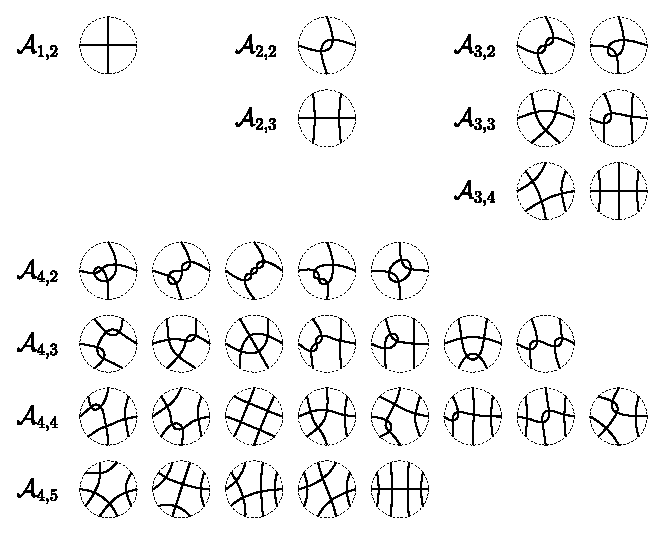
\includegraphics[scale=0.8]{c/alternating-tangles-1-4.eps}
			\caption{\footnotesize Альтернированные танглы до 4-х перекрестков.\label{figure:tangles14}}
		\end{figure}

		\begin{figure}[ht]
			\centering
			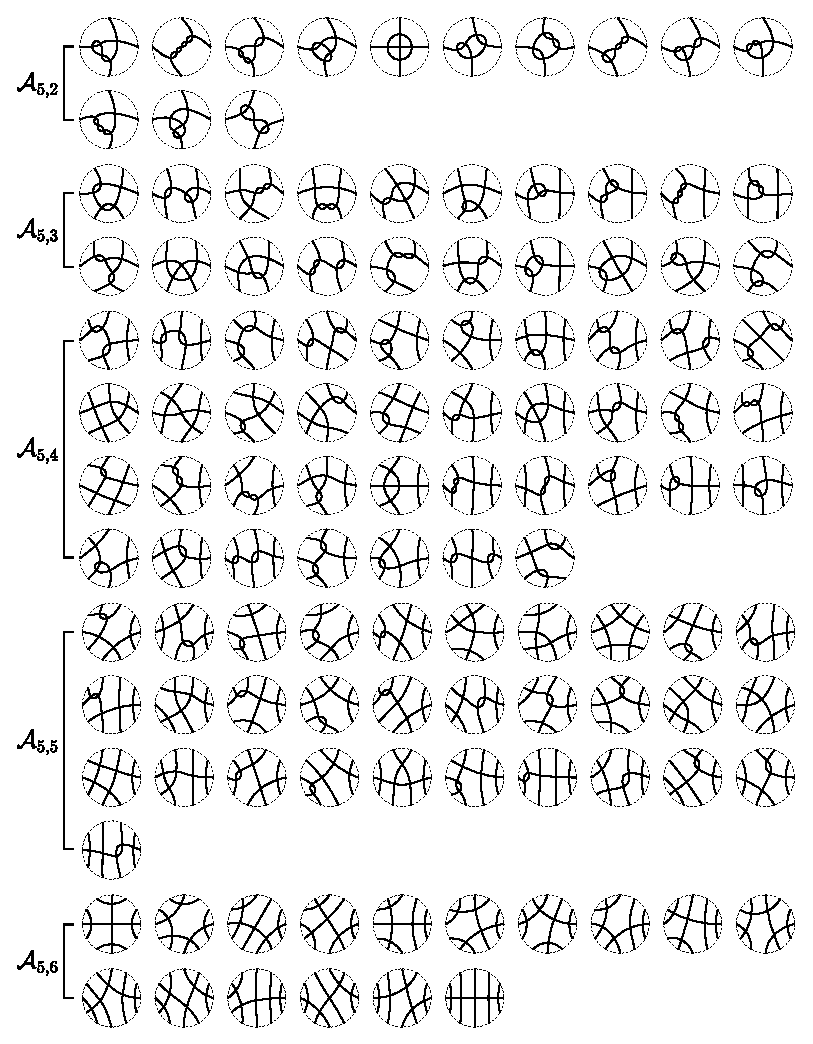
\includegraphics[scale=0.8]{c/alternating-tangles-5.eps}
			\caption{\footnotesize Альтернированные танглы до 5-ю перекрестками.\label{figure:tangles5}}
		\end{figure}

		Отметим, что число альтернированных $k$-танглов растет с увеличением числа перекрестков гораздо быстрее, нежели число
		альтернированных зацеплений~\cite{RankinSchermannSmith2002_1, RankinSchermannSmith2002_2, RankinSmith2002}. Например, различных
		зацеплений с 12 перекрестками всего 3308, и даже для $n = 19$ зацеплений получается меньше, чем $k$-танглов при $n = 12$.

	\newpage
	\section{Неальтернированные $k$-танглы}\label{section:non-alternating}

		Задача перечисления произвольных узлов, зацеплений и, соответственно, $k$-танглов является гораздо более сложной, чем аналогичная
		для альтернированного случая, и все известные на данный момент общие алгоритмы неприменимы из-за непрактичного времени работы. Даже
		для узлов самая большая на данный момент таблица~\cite{HosteThistlethwaiteWeeks1998} построена скорее с помощью ad hoc приемов и
		аккуратного программирования, а не какого-то общего алгоритма. Связано это с тем, что, хотя движения
		Рейдемейстера (см.~\figureref{figure:reidemeister-moves}) позволяют из любой диаграммы зацепления или $k$-тангла получить любую другую
		возможную его диаграмму, но в процессе преобразования может произойти увеличение числа перекрестков. Некоторые оценки на общее
		число движений известны~\cite{HassLagarias2001, Hayashi2005}, но полный перебор по-прежнему остается слишком трудоемким.

		\begin{figure}[ht]
			$$
			\def\pica#1{\raise-4mm\hbox{\protect\includegraphics[origin=c]{reidemeister.#1.eps}}}
			\pica{11}\ \backsimeq\ \pica{12}\qquad
			\pica{21}\ \backsimeq\ \pica{22}\qquad
			\pica{31}\ \backsimeq\ \pica{32}
			$$
			\caption{\footnotesize Движения Рейдемейстера.\label{figure:reidemeister-moves}}
		\end{figure}

		Как следствие, мы так просто уже не можем по диаграмме сказать, является ли она минимальной по числу перекрестков, а нашей задачей
		при перечислении является как раз нахождение для каждого $k$-тангла одной из его минимальных диаграмм. Более того, даже зная одну
		из минимальных диаграмм $k$-тангла, мы не можем просто узнать все остальные его минимальные диаграммы, поскольку какого-то набора
		движений, позволяющих получать друг из друга все возможные минимальные диаграммы, на данный момент неизвестно.

		Подобно использованному для узлов в~\cite{HosteThistlethwaiteWeeks1998}, наш метод перечисления произвольных $k$-танглов
		также состоит из трех шагов: генерирования некоторого множества диаграмм с перекрестками, удаления из полученного множества
		дубликатов c помощью движений Рейдемейстера и некоторого набора более сложных преобразований (которые, разумеется, представляются в
		виде нескольких последовательных движений Рейдемейстера, но значительно облегчают нам задачу) и, наконец, анализа получившихся
		диаграмм с помощью топологических инвариантов.

		Следующие три параграфа описывают три этих этапа соответственно. Затем следуют некоторые результаты с замечаниями.

	\subsection{Генерация диаграмм}

		Ранее мы уже научились собирать альтернированные диаграммы $k$-танглов из макроперекрестков со сложной внутренней структурой и
		нетривиальной симметрией. Подобный подход может быть использован и для генерации диаграмм с произвольными состояниями перекрестков:
		единственным макроперекрестком здесь будет ``перекресток со знаком'', группой симметрии которого будет $DS$ (в
		терминах~\figureref{figure:D4-subgroups}). Таким образом мы сразу получаем все возможные простые связные диаграммы $k$-танглов.

		Однако, в получаемом таким образом множнстве практически для любой диаграммы находится отличающаяся от нее только сменой знаков
		всех ее перекрестков, что приводит к практически двухкратному разрастанию всего множества и от чего хотелось избавится. Введем
		для этого \textit{группу глобальных преобразований}, то есть подгруппу $D_4$, любой элемент которой может быть применен ко всем
		макроперекресткам (но один и тот же элемент ко всем), а результат применения объявляется эквивалентным исходной диаграмме. В нашем
		случае такой группой может быть, например, $ECS$, элемент $EC$ которой обращает знак перекрестка. Теперь при вычислении \RCD{} мы
		будем брать лексикографический минимум по всем возможным применениям группы глобальных преобразований. Математически это означает,
		что мы заменили группу преобразований диаграммы $k$-тангла с $D_{2k}$ на ее декартово произведние на группу глобальных преобразований.
		Так как фактически ничего в обосновании алгоритма не поменялось, то он и в таком случае будет работать и давать правильный результат.

		Также нам хотелось бы избавится от диаграмм, которые немедленно упрощаются вторым движением Рейдемейстера (диаграмм, упрощающихся
		первым движением Рейдемейстера не будет, благодаря простоте). Для этого заметим, что свойство диаграммы упрощатся таким образом
		является наследуемым, что немедленно приводит к простой модификации алгоритма, решающей проблему. Для примера количества таких
		диаграмм с не более, чем 10 перекрестками, приведены в Таблице~\ref{table:tangle-diagrams}.

		\begin{table}[ht]
			\caption{Количество диаграмм $k$-танглов с $n$ перекрестками\label{table:tangle-diagrams}}
			\centering
			\begin{tabular}{|c||r|r|r|r|r|r|r|r|r|r|}
			\hline
			$k$\textbackslash $n$
			    & 1 & 2 &  3 &   4 &   5 &       6 &        7 &           8 &            9 &            10 \\
			\hline\hline
			2   & 1 & 1 &  3 &  14 &  76 &     486 &   3\,544 &     28\,357 &     239\,061 &   2\,094\,320 \\
			3   & . & 2 &  4 &  25 & 148 &  1\,146 &   9\,036 &     76\,696 &     670\,368 &   6\,027\,768 \\
			4   & . & . &  6 &  33 & 258 &  2\,125 &  18\,537 &    165\,895 &  1\,518\,645 &  14\,133\,545 \\
			5   & . & . &  . &  32 & 290 &  3\,086 &  30\,276 &    298\,392 &  2\,919\,788 &  28\,649\,272 \\
			6   & . & . &  . &   . & 206 &  3\,081 &  38\,515 &    435\,907 &  4\,726\,468 &  50\,026\,435 \\
			7   & . & . &  . &   . &   . &  1\,718 &  33\,645 &    490\,784 &  6\,223\,320 &  73\,693\,696 \\
			8   & . & . &  . &   . &   . &       . &  15\,722 &    380\,276 &  6\,298\,284 &  88\,352\,732 \\
			9   & . & . &  . &   . &   . &       . &        . &    154\,656 &  4\,376\,155 &  81\,234\,008 \\
			10  & . & . &  . &   . &   . &       . &        . &           . &  1\,580\,929 &  51\,154\,784 \\
			11  & . & . &  . &   . &   . &       . &        . &           . &            . &  16\,656\,936 \\
			\hline
			all & 1 & 3 & 13 & 104 & 978 & 11\,642 & 149\,275 & 2\,030\,963 & 28\,553\,018 & 412\,023\,496 \\
			\hline
			\end{tabular}
		\end{table}

	\subsection{Движения}

		После того, как мы научились получать диаграммы $k$-танглов, будем действовать следующим образом: поддерживать с помощью
		систем непересекающихся множеств~\cite{CormenLeisersonRivestStein2009, Sedgewick1983} на них соотношение эквивалентности, для
		каждой из диаграмм объявляя эквивалентными ей те, которые могут быть получены из нее применением одного из движений, о которых
		речь пойдет ниже, и затем, если возможно, то уменьшением числа перекрестков с помощью первого и второго движений Рейдемейстера
		жадным образом (легко показать, что результат такой жадной редукции не зависит от выбора порядка применяемых движений). Сами
		диаграммы мы здесь идентифицируем с помощью видоизмененного, как в предыдущем параграфе, \RC{}.

		Хотя такая схема приводит к большому расходу памяти и не может быть использована в действительно объемном перечислении, но это
		в данном случае не является проблемой и даже дает некоторые преимущества, так как, во-первых, лимитирующим фактором перечисления,
		как будет понятно из дальнейшего, является сила используемых для доказательства различности полученных классов эквивалентности
		топологических инвариантов, и, во-вторых, подход позволяет ``заглянуть вперед'' по количеству перекрестков и обнаружить пары
		эквивалентных диаграмм, которые не объединились с помощью только набора движений, что может служить подсказками для изобретения
		новых более сложных движений.

		\begin{figure}[ht]
			\centering
			$$
			{\raise-4mm\hbox{\protect\includegraphics{pass.1.eps}}}
			\qquad
			{\raise-5mm\hbox{\protect\includegraphics{pass.2.eps}}}
			$$
			\caption{\footnotesize Pass.\label{figure:pass}}
		\end{figure}

		В качестве собственно движений мы будем использовать третье преобразование Рейдемейстера, уже упоминавшийся выше flype, а также
		pass, являющийся обобщением третьего преобразования Рейдемейстера --- давно известное движение (первые составители таблиц узлов
		предполагали, что пары из flype и pass достаточно, чтобы показать эквивалентность любой пары минимальных диаграмм любого узла).
		Следует, однако, заметить, что в, отличие от узлов, для $k$-танглов существует два возможных варианта движения pass
		(см.~\figureref{figure:pass}).

	\subsection{Инварианты}

		Последним шагом к перечислению неальтернированных $k$-танглов является доказательство того, что полученные на предыдущем шаге
		классы эквивалентности соответствуют действительно неэквивалентным $k$-танглам. Для этого мы используем модификацию полинома
		Джонса~\cite{Jones2005}, заключающуюся в сведении диаграммы всеми возможными способами с помощью скейн-соотношений:

		$$
		\begin{aligned}
			& \langle \ell \rangle = a\langle \ell_1 \rangle + \frac{1}{a} \langle {\ell_2} \rangle \\
			& \langle {\ell{\textstyle{}\bigcup{}}\bigcirc} \rangle = -\left( a^2 + \frac{1}{a^2} \right) \langle \ell \rangle \\
			& 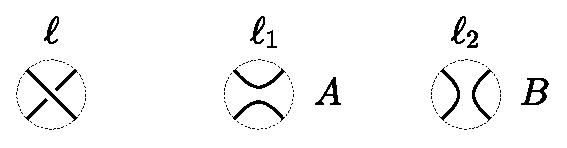
\includegraphics[scale=0.5]{c/kauffman-skein-definition.eps}
		\end{aligned}
		$$

		к некоторому множеству диаграмм без перекрестков (см.~\figureref{figure:jones-example}). Очевидно, что для $k$-тангла множество этих
		простейших диаграмм имеет взаимно однозначное соответствие с множеством правильных скобочных последовательностей длинны $2 k$. Таким
		образом полученный инвариант принимает значения в модуле над полиномами Лорана с базисом из правильных скобочных последовательностей.
		С симметриями, связанными с поворотами и отражениями можно разобраться следующим образом: применим соответствующие преобразования к
		элементам базиса, и, введя лексикографический порядок на полиномах, возьмем минимальный результат.

		\begin{figure}[ht]
			\centering
			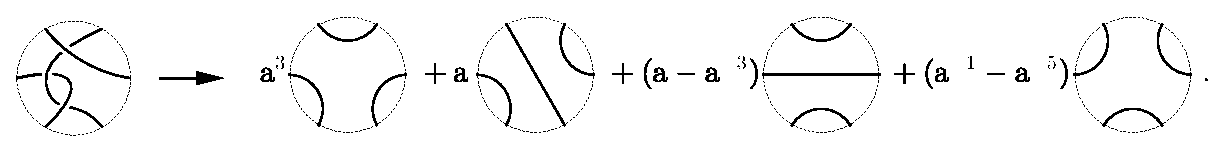
\includegraphics[scale=0.7]{c/tangle-kauffman-example.eps}
			\caption{\footnotesize Пример применения скейн-соотношений.\label{figure:jones-example}}
		\end{figure}

		Полученный инвариант гарантированно дает коллизии на диаграммах, отличающихся некоторым аналогичным мутации преобразованием, что в
		случае $k$-танглов начинается со значительно меньшего, чем для узлов, количества перекрестков. Поэтому, чтобы его немного усилить,
		мы будем его вычислять от всех возможных подмножеств нитей диаграммы и сравнивать результаты как множества.

	\subsection{Результаты}

		\begin{table}[ht]
			\caption{Количество $k$-танглов с $n$ перекрестками.\label{table:non-alternating-tangles}}
			\centering
			\let\ul=\underline
			\begin{tabular}{|c||r|r|r|r|r|r|r|r|}
			\hline
			$k$\textbackslash $n$
			    & 1 & 2 &  3 &  4 &   5 &      6 &        7 &           8 \\
			\hline\hline
			2   & 1 & 1 &  2 &  6 &  15 &     47 &      156 &    \ul{589} \\
			3   & . & 2 &  4 & 15 &  48 &    201 & \ul{811} & \ul{3\,755} \\
			4   & . & . &  6 & 30 & 154 &    762 &   3\,796 &     19\,468 \\
			5   & . & . &  . & 32 & 258 & 1\,916 &  11\,931 &     71\,943 \\
			6   & . & . &  . &  . & 206 & 2\,717 &  24\,735 &    186\,790 \\
			7   & . & . &  . &  . &   . & 1\,718 &  29\,572 &    323\,781 \\
			8   & . & . &  . &  . &   . &      . &  15\,722 &    333\,764 \\
			9   & . & . &  . &  . &   . &      . &        . &    154\,656 \\
			\hline
			all & 1 & 3 & 12 & 83 & 681 & 7\,361 &  86\,724 & 1\,094\,746 \\
			\hline
			\end{tabular}
		\end{table}

		\begin{figure}[ht]
			\centering
			\includegraphics[scale=0.8]{nonalternating-tangles.1.eps}
			\caption{\footnotesize Неальтернированные $k$-танглы до 4-х перекрестков.\label{figure:nonalternating-tangles-4}}
		\end{figure}

		\begin{figure}[ht]
			\centering
			\includegraphics[scale=0.8]{nonalternating-tangles.2.eps}
			\caption{\footnotesize Некоторые другие неальтернированные $k$-танглы.\label{figure:nonalternating-tangles-rest}}
		\end{figure}

		\begin{table}[ht]
			\caption{Количество слабо эквивалентных $k$-танглов с $n$ перекрестками.\label{table:weak-tangles}}
			\centering
			\begin{tabular}{|c||r|r|r|r|r|}
			\hline
			$k$\textbackslash $n$
			    & 4 & 5 & 6 &  7 &   8 \\
			\hline\hline
			2   & 1 & 2 & 8 & 29 & 132 \\
			3   & . & . & 1 &  2 &  14 \\
			4   & . & . & . &  . &  16 \\
			\hline
			all & 1 & 2 & 9 & 31 & 162 \\
			\hline
			\end{tabular}
		\end{table}

		\begin{figure}[ht]
			\centering
			\includegraphics[scale=0.8]{nonalternating-tangles.3.eps}
			\caption{\footnotesize $k$-танглы до 7 перекрестков с точностью до слабой эквивалентности.\label{figure:weak-tangles-7}}
		\end{figure}

		Количества $k$-танглов до 8 перекрестков приведены в Таблице~\ref{table:non-alternating-tangles}. Все числа, кроме подчеркнутых,
		доказаны с использованием полинома Джонса. Подчеркнутые значения проверены с помощью ``заглядывания вперед'', что однако не
		может считаться доказательством.

		Изображения некоторых неальтернированных $k$-танглов приведены на \figureref{figure:nonalternating-tangles-4} и
		\figureref{figure:nonalternating-tangles-rest}.

		Также мы пытались повторить результаты~\cite{KanenobuSaitoSatoh2003}, где были вручную перечислены $2$-танглы не более чем
		с 7 перекрестками с точностью до слабой эквивалентности. Получившиеся количества и некоторые диаграммы приведены в
		Таблице~\ref{table:weak-tangles} и на~\figureref{figure:weak-tangles-7} соответственно. Следует отметить, что для 7
		перекрестков у нас получилось на один $2$-тангл больше, чем в~\cite{KanenobuSaitoSatoh2003}.
%		``Лишним'' является предпоследний
%		в первом ряду $2$-тангл из соответствующей группы на~\figureref{figure:weak-tangles-7}.

		Исходный код программы на \texttt{Haskell}, используемой нами при перечислении, можно найти в открытом репозитории по
		адресу \texttt{https://github.com/mishun/tangles}.

	\newpage
	\begin{thebibliography}{88}

		\bibitem{BogdanovMeshkovOmelchenkoPetrov2011}
		{\em Bogdanov~A., Meshkov~V., Omelchenko~A., Petrov~M.}
		Classification of $k$-tangle projections using cascade representation.
		Journal of Knot Theory and Its Ramifications, to appear.
		e-print: \texttt{arXiv:0712.3859v2}

		\bibitem{Conway1970}
		{\em Conway~J.}
		An enumeration of knots and links, and some of their algebraic properties.
		Computational Problems in Abstract Algebra (John Leech, ed.), Pergamon Press, Oxford
		and New York, 1969, 329--358.

		\bibitem{CormenLeisersonRivestStein2009}
		{\em Cormen~T., Leiserson~C., Rivest~R., Stein~C.}
		Introduction to Algorithms (3rd ed.).
		MIT Press., 2009.

		\bibitem{Cromwell2004}
		{\em Cromwell~P.}
		Knots and links.
		Cambridge university press, 2004, 350\,с.

		\bibitem{Jones2005}
		{\em Jones~V.}
		The Jones Polynomial.
		\texttt{http://www.math.berkeley.edu/\textasciitilde vfr/jones.pdf}

		\bibitem{HassLagarias2001}
		{\em Hass~J., Lagarias~J.}
		The number of Reidemeister moves needed for unknotting.
		J. Amer. Math. Soc. 14 (2001), no. 2, 399--428

		\bibitem{Hayashi2005}
		{\em Hayashi~C.}
		The number of Reidemeister moves for splitting a link.
		Math. Ann., 2005, Vol.\,332, {\bf 2}, 239--252.

		\bibitem{HosteThistlethwaiteWeeks1998}
		{\em Hoste~J., Thistlethwaite~M., Weeks~J.}
		The first 1,701,936 knots.
		Math. Intelligencer, 1998, Vol.\,20, {\bf 4}, 33--48 (1998).

		\bibitem{KanenobuSaitoSatoh2003}
		{\em Kanenobu~T., Saito~H., and Satoh~S.}
		Tangles with up to seven crossings.
		Interdisciplinary Information Sciences, 2003, Vol.\,9, {\bf 1}, 127--140.

		\bibitem{Kauffman1987}
		{\em Kauffman~L.~H.}
		State Models and the Jones Polynomial.
		Topology, 1987, {\bf 26}, 395--407.

		\bibitem{KauffmanLambropoulou2004}
		{\em Kauffman~L., Lambropoulou~S.}
		On the classification of rational tangles.
		Advances in Applied Mathematics, 2004, {\bf 2}, 199--237.
		e-print:~\texttt{arXiv:math/0311499v2}.

		\bibitem{McKay1998}
		{\em McKay~B.~D.}
		Isomorph-free exhaustive generation.
		J. Algorithms, 1998, {\bf 26}, 306--324.

		\bibitem{MenascoThistlethwaite1991}
		{\em Menasco~W., Thistlethwaite~M.}
		The Tait Flyping Conjecture.
		Bull. Amer. Math. Soc., 1991, {\bf 25}, 403--412.

		\bibitem{MenascoThistlethwaite1993}
		{\em Menasco~W., Thistlethwaite~M.}
		The Classification of Alternating Links.
		Ann. Math., 1993, {\bf 138}, 113--171.

		\bibitem{Murasugi1987_1}
		{\em Murasugi~K.}
		The Jones Polynomial and Classical Conjectures in Knot Theory.
		Topology, 1987, {\bf 26}, 187--194.

		\bibitem{Murasugi1987_2}
		{\em Murasugi~K.}
		Jones Polynomials and Classical Conjectures in Knot Theory II.
		Math. Proc. Cambridge Philos. Soc., 1987, {\bf 102}, 317--318.

		\bibitem{RankinSchermannSmith2002_1}
		{\em Rankin~S., Schermann~J., Smith~O.}
		Enumerating the prime alternating knots, Part I,
		Journal of Knot Theory and Its Ramifications, 2004, Vol.\,13, {\bf 1}, 57--100.
		e-print:~\texttt{arXiv:math/0211346}

		\bibitem{RankinSchermannSmith2002_2}
		{\em Rankin~S., Schermann~J., Smith~O.}
		Enumerating the prime alternating knots, Part II,
		Journal of Knot Theory and Its Ramifications, 2004, Vol.\,13, {\bf 1}, 101--149.
		e-print:~\texttt{arXiv:math/0211348}

		\bibitem{RankinSmith2002}
		{\em Rankin~S., Smith~O.}
		Enumerating the Prime Alternating Links.
		Journal of Knot Theory and Its Ramifications, 2004, Vol.\,13, {\bf 1}, 151--173.
		e-print:~\texttt{arXiv:math/0211451}

		\bibitem{Sedgewick1983}
		{\em Sedgewick~R.}
		Algorithms (1st ed.).
		Addison-Wesley, 1983.

		\bibitem{SundbergThistlethwaite1998}
		{\em Sundberg~C., Thistlethwaite~M.}
		The Rate of Growth of the Number of Prime Alternating Links and Tangles.
		Pacific Journal of Mathematics, 1998, Vol.\,182, {\bf 2}, 329--358.

		\bibitem{Tait1900}
		{\em Tait~P.~G.}
		On Knots I, II, III.
		Scientific Papers.
		London: Cambridge University Press, 1900, Vol.\,1, 273--347.

		\bibitem{Thistlethwaite1987}
		{\em Thistlethwaite~M.}
		A Spanning Tree Expansion of the Jones Polynomial.
		Topology, 1987, {\bf 26}, 297--309. 

		\bibitem{Thistlethwaite1988}
		{\em Thistlethwaite~M.}
		Kauffman's Polynomial and Alternating Links.
		Topology, 1988, {\bf 27}, 311--318.

		\bibitem{JustinZuber2003}
		{\em Zinn-Justin~P., Zuber~J.}
		Matrix integrals and the generation and counting of virtual tangles and links.
		Journal of Knot Theory and Its Ramification, 2004, Vol.\,13, {\bf 2}, 325--356.
		e-print:~\texttt{arXiv:math-ph/0303049}.

	\end{thebibliography}
\end{document}
